\subsubsection{Objective}
The third research question investigates how the installation dates and operational periods of weather stations affect data availability over time and across Austrian regions and elevation zones. The goal is to identify spatial and temporal coverage gaps, also referred to as ``data deserts,'' that could affect the interpretation of long-term climate analyses.

\subsubsection{Methodology}

To address this question, the implementation proceeded in two main steps:

\begin{enumerate}
  \item \textbf{Metadata-Based Coverage Matrix:}  
    Using station metadata (installation and deactivation dates), a year-by-year activity matrix from 1970 to 2025 was constructed via a cross join with the full year range. Only periods when stations were active were retained. Each station was then categorized into one of five elevation zones (as in RQ1). Aggregated counts by year, elevation zone, and federal state were used to provide a theoretical view of station availability.

  \item \textbf{Real Measurement-Based Coverage:}  
    To assess actual data availability, the climate dataset was filtered to include only records with at least one valid measurement. These were grouped using the same year–elevation–region schema as the metadata-based matrix.
\end{enumerate}

In this report, the results are shown for the Lower-Alps zone (1000–1499 m). Results for the other four zones are available in the accompanying Jupyter Notebook.

\subsubsection{Results and Interpretation}

\paragraph{Figure~\ref{fig:coverage_meta_loweralps}: Metadata-Based Coverage (Lower Alps)}  
The heat map shows that Carinthia, Salzburg, and Styria have maintained a consistent network of 7 to 16 active stations per year since the 1970s. In contrast, regions such as Lower Austria and Upper Austria are either absent or only sporadically represented in this altitude zone. Vorarlberg shows moderate coverage from around 2008 onward, while Tyrol stands out with a well-developed and continuous station network throughout the entire period.

\begin{figure}[ht]
  \centering
    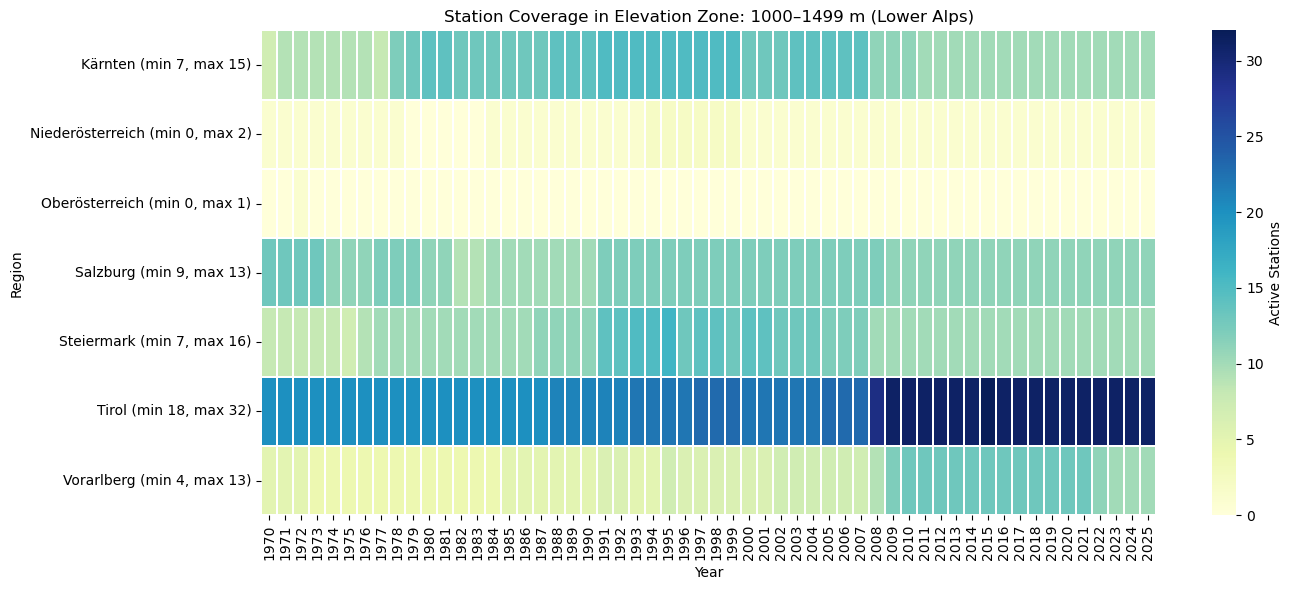
\includegraphics[width=0.45\textwidth]{img/coverage_zone_loweralps_meta.png}
    \caption{Metadata-based station coverage in elevation zone: 1000--1499\,m (Lower Alps)}
    \label{fig:coverage_meta_loweralps}
\end{figure}

\paragraph{Figure~\ref{fig:coverage_real_loweralps}: Actual Measurement-Based Coverage (Lower Alps)}  
The second heatmap confirms that actual measurement coverage aligns closely with the metadata. Again, Tyrol is best represented, while several eastern federal states exhibit minimal or no active data-producing stations in this elevation zone.

\begin{figure}[ht]
  \centering
    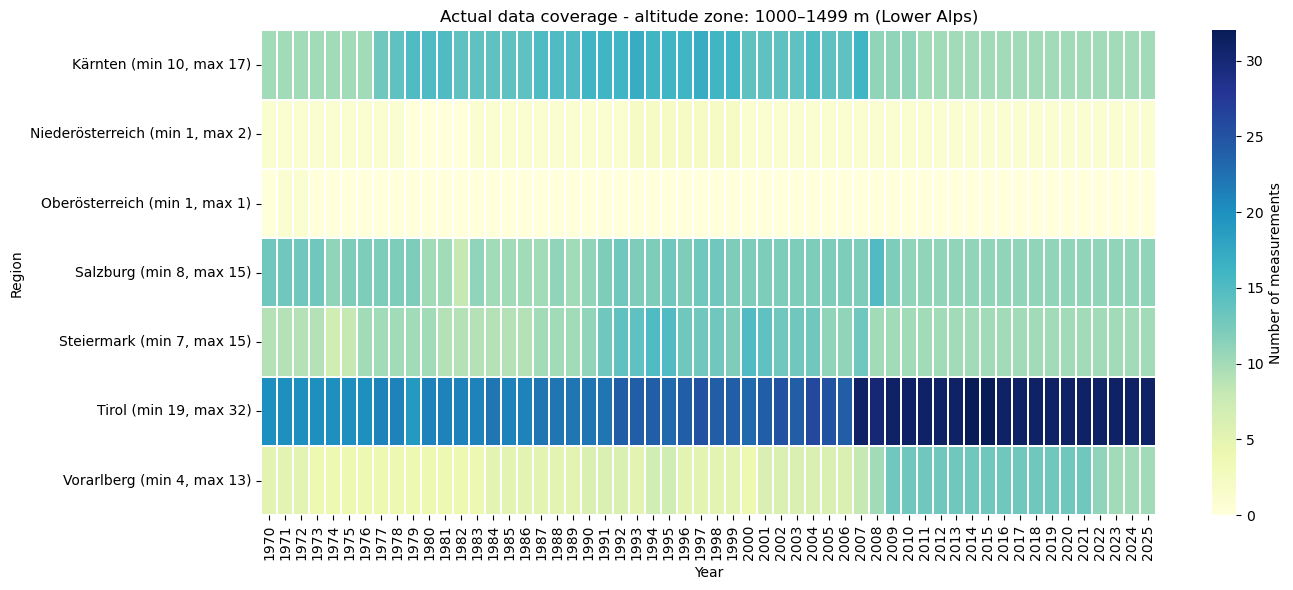
\includegraphics[width=0.45\textwidth]{img/data_coverage_loweralps.png}
    \caption{Actual measurement-based coverage in elevation zone: 1000--1499\,m (Lower Alps)}
    \label{fig:coverage_real_loweralps}
\end{figure}

\subsubsection{Conclusion}
Both the metadata-based and measurement-based heat maps confirm persistent long-term data gaps in the Lower Alps (1000–1499 m), particularly in Upper and Lower Austria.

In other elevation zones as well, the two coverage representations generally agree. However, minor differences in shading between the two heat maps reveal important nuances: lighter shading in the measurement maps compared to metadata suggests technically active stations with little or incomplete data. Conversely, darker shading in the measurement maps may indicate incorrect metadata or other data quality issues.

These findings underline the importance of validating metadata-based assumptions against actual measurement data—especially for high-resolution analyses or policy-relevant climate studies.